\section{Our computational model of serendipity} \label{sec:background}

Summarising the criteria discussed earlier, we propose the following
definition, expressed in two phases: discovery and invention.  The
definition centres on the four components of serendipity, outlined
above, which can subsequently be made sense of and evaluated with
reference to the four dimensions of serendipity.  These, in turn, are
understood to be embedded in an environment exhibiting many, but not
necessarily all, of the environmental factors listed above.

\begin{quote}
\begin{enumerate}[itemsep=2pt,labelwidth=9em,leftmargin=6em,rightmargin=2em]
\item[\emph{(\textbf{1 - Discovery})}] \emph{Within a system with a prepared mind, a previously uninteresting serendipity trigger arises due to circumstances that the system does not control, and is classified as interesting by the system; and,}
\item[\emph{(\textbf{2 - Invention})}] \emph{The system, by subsequently processing this trigger and background information together with relevant reasoning, networking, or experimental techniques, obtains a novel result that is evaluated favourably by the system or by external sources.}
\end{enumerate}
\end{quote}

This can be summarised schematically as follows:

% \begingroup
\tikzset{
block/.style = {draw, fill=white, rectangle, minimum height=3em, minimum width=3em},
tmp/.style  = {coordinate}, 
sum/.style= {draw, fill=white, circle, node distance=1cm},
input/.style = {coordinate},
output/.style= {coordinate},
pinstyle/.style = {pin edge={to-,thin,black}}
}

\begin{tikzpicture}[auto, node distance=2cm,>=latex']
    \node [sum] (sum1) {};
    \node [input, name=pinput, above left=.7cm and .7cm of sum1] (pinput) {};
    \node [input, name=tinput, left of=sum1] (tinput) {};
    \node [input, name=minput, below left of=sum1] (minput) {};
    \node [input, name=minput, right of=sum1] (moutput) {};
    \draw [->] (pinput) -- node{$p$} (sum1);
    \draw [->] (tinput) -- node{\vphantom{{\tiny g}}$T$} (sum1);
    \draw [->] (sum1) -- node{\vphantom{{\tiny g}}$T^{\star}$}  (moutput);
\end{tikzpicture}
\hspace{1cm}
\begin{tikzpicture}[auto, node distance=2cm,>=latex']
    \node [sum] (sum1) {};
    \node [input, name=pinput, above left=.7cm and .7cm of sum1] (pinput) {};
    \node [input, name=tinput, left of=sum1] (tinput) {};
    \node [input, name=minput, below left of=sum1] (minput) {};
    \node [sum, right of=sum1] (sum2) {};
    \node [input, name=minput, right of=sum2] (moutput) {};
    \draw [->] (pinput) -- node{$p^{\prime}$} (sum1);
    \draw [->] (tinput) -- node{\vphantom{{\tiny g}}$T^{\star}$} (sum1);
    \draw [->] (sum1) -- node{\vphantom{{\tiny g}}$R$} (sum2);
    \draw [->] (sum2) -- node{$|R|>0$}  (moutput);
\end{tikzpicture}
\endgroup


{\centering
\includegraphics[width=.8\textwidth]{schematic}
\par}

\includegraphics{figures/schematic/schematic.png}

